\subsection{Java Dependency Management}
Prima di tutto è necessario indicare in che linguaggio il nostro progetto viene rilasciato (consideriamo d'ora in poi solo il caso di Java), per farlo aggiungiamo in testa al file build.gradle:
\begin{lstlisting}[frame=single]
apply plugin: 'java' \end{lstlisting}
A questo punto per poter usufruire di una dipendenza è necessario specificare da dove Gradle deve andare a prenderla, dobbiamo quindi indicare il repository remoto di riferimento. Se per esempio vogliamo che il nostro repository di riferimento sia Maven allora dobbiamo aggiungere al build.gradle:
\begin{lstlisting}[frame=single]
repositories {
    mavenCentral()
} \end{lstlisting}
In questo modo tutte le dipendenze che andremo a indicare successivamente saranno riferimenti alle pubblicazioni su Maven Central. La dichiarazione delle dipendenze deve essere inserita nel tag \texttt{dependencies} nel build.gradle file. Per esempio vogliamo avere junit 4.12 come dipendenza al nostro progetto Gradle allora dobbiamo aggiungere:
\begin{lstlisting}[frame=single]
dependencies {
    testImplementation group: 'junit', name: 'junit', version: '4.12' 
} \end{lstlisting}
Osserviamo che nella dichiarazione ci sono 4 diversi indicatori:
\begin{itemize}
    \item \texttt{testImplementation} indica la configurazione della dipendenza, in questo caso sarà importata durante l'implementazione dei test;
    \item \texttt{group, name, version} corrispondono rispettivamente al groupId (nome del team o della società che ha sviluppato il modulo), artifactId (nome effettivo del modulo) e al version (versione del modulo) definiti su Maven.
\end{itemize}
Esiste un modo molto più diretto per indicare una dipendenza:
\begin{lstlisting}[frame=single]
dependencies {
    testImplementation 'junit:junit:4.12'
} \end{lstlisting}
Ha lo stesso significato precedente ma ha una forma più compatta, forma che adotta anche la documentazione Maven:
\begin{figure}[H]
\centering
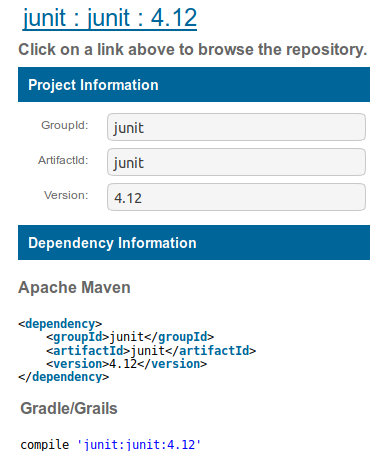
\includegraphics[width=0.4\linewidth]{3DependencyManagement/javaDep/gradleInMavenRepo.png}
\end{figure}
Spesso in un progetto non è necessario specificare il numero dell'aggiornamento della versione, ma basta la versione più aggiornata, questo è possibile indicarlo a gradle con un \texttt{+} subito dopo la versione voluta:
\begin{lstlisting}[frame=single]
dependencies {
    testImplementation 'junit:junit:4.+'
} \end{lstlisting}
In questo modo quando eseguiremo il task \texttt{dependencies} gradle si assicurerà che la versione in uso di quella dipendenza specifica sia l'ultima rilasciata. Possiamo notare ora la differenza sostanziale della configurazione delle dipendenze tra il pom.xml di Maven e il build.gradle di Gradle. A questo punto per scaricare le dipendenze si deve eseguire il comando \texttt{dependencies} il cui output restituirà una lista di tutte le configurazioni con le relative dipendenze associate (non mostro tutto l'output perchè è molto corposo):
\begin{verbatim}
> Task :dependencies 

------------------------------------------------------------
Root project
------------------------------------------------------------

[...]

compile - Dependencies for source set 'main' (deprecated, use 'implementation ' instead).
No dependencies

[...]

default - Configuration for default artifacts.
No dependencies

[...]

runtime - Runtime dependencies for source set 'main' (deprecated, use 'runtimeOnly ' instead).
No dependencies

[...]

testCompileClasspath - Compile classpath for source set 'test'.
\--- junit:junit:4.+ -> 4.12
     \--- org.hamcrest:hamcrest-core:1.3

testCompileOnly - Compile only dependencies for source set 'test'.
No dependencies

testImplementation - Implementation only dependencies for source set 'test'. (n)
\--- junit:junit:4.+ (n)

testRuntime - Runtime dependencies for source set 'test' (deprecated, use 'testRuntimeOnly ' instead).
No dependencies

testRuntimeClasspath - Runtime classpath of source set 'test'.
\--- junit:junit:4.+ -> 4.12
     \--- org.hamcrest:hamcrest-core:1.3

[...]


BUILD SUCCESSFUL in 0s
1 actionable task: 1 executed \end{verbatim}
Come è possibile notare dall'output esistono molte configurazioni associabili a una dipendenza: compile, default, runtime, testImplementation, e così via, ognuno dei ha uno scopo ben preciso. Possiamo dividere le configurazioni in 3 scopi principali:
\begin{enumerate}
    \item implementation
    \item api
    \item testImplementation
\end{enumerate}
% pagina 63 https://docs.gradle.org/current/userguide/userguide.pdf